\chapter{Simulation}
\label{simulation}
\nomenclature{DOF}{Degree of freedom}
A 6-DOF flight simulator was used to validate the drag prediction method before hardware was purchased. The main utility of the simulator was to provide simulated flight test data with signals that contained no errors. The actual sensors used for flight testing contain noise, and this noise can be added onto the pure simulator signals to test the sensitivity of the drag polar regression to sensor accuracy.

\section{Simulation Environment}
The flight simulator used was a model of the de Haviland Beaver that comes as a demo in the Aerospace Toolbox of Simulink. The Simulink model was modified to output required signals to the workspace, which essentially created a sensor with zero noise. The mass, moments of inertia, and reference lengths were then scaled to those of a Zagi R/C aircraft\cite{stevens2003aircraft}. The original Simulink model was already connected to a FlightGear Flight Sim, used as a visualization engine. This model was slightly altered to make flight gauges function properly.

\section{Simulation Inputs}
The engine forces and moments were set to zero in the simulator, to match the assumption of a folding propeller. The drag force calculation built into the Beaver Simulink model was replaced with a parabolic drag polar of the form

\begin{align}
C_D &= C_{D_0} + K_1(C_L(\alpha)-C_{L_{min}})^2+\frac{(C_L(\alpha))^2}{\pi eAR}
\end{align}
\nomenclature{$AR$}{Aspect ratio}
\nomenclature{$C_L$}{Lift coefficient}
\nomenclature{$C_D$}{Drag coefficient}
\nomenclature{e}{Wing lift distribution}
\nomenclature{$C_{D_0}$}{Parasite drag coefficient}
\nomenclature[G]{$\alpha$}{Angle of attack}
Airfoil data, including $K_1$, $C_{L_{min}}$, and $C_L(\alpha)$, was taken from nonlinear aerodynamic data of a NACA 0012\cite{osborne2007transitions}. While this approximation to a real drag polar does not capture the nonlinear section of profile drag rise due to stall, it does represent the limited lifting capability of a real wing.

\section{Simulation Results}
The first goal of the simulation testing was to verify the drag polar equations were correct, and that the data analysis routines developed in MATLAB did in fact match inputs to outputs. The simulation was initialized with various initial states to ensure there was no dependency on initial conditions. The vehicle was then flown by an R/C aircraft pilot using a joystick attached to the simulation. It was noted early in the simulation testing that flying a sweep of speeds was beneficial, as a wider range of the drag polar was flown. This result was included in much of the flight test planning. 

After adequate data had been taken, the data was analyzed without adding simulated sensor noise. The results in Figure \ref{dragPolarNoNoise} show that the equations of motion used in the data analysis functions properly calculate the coefficients being passed into the system.

\begin{figure}[H]
  \centering
    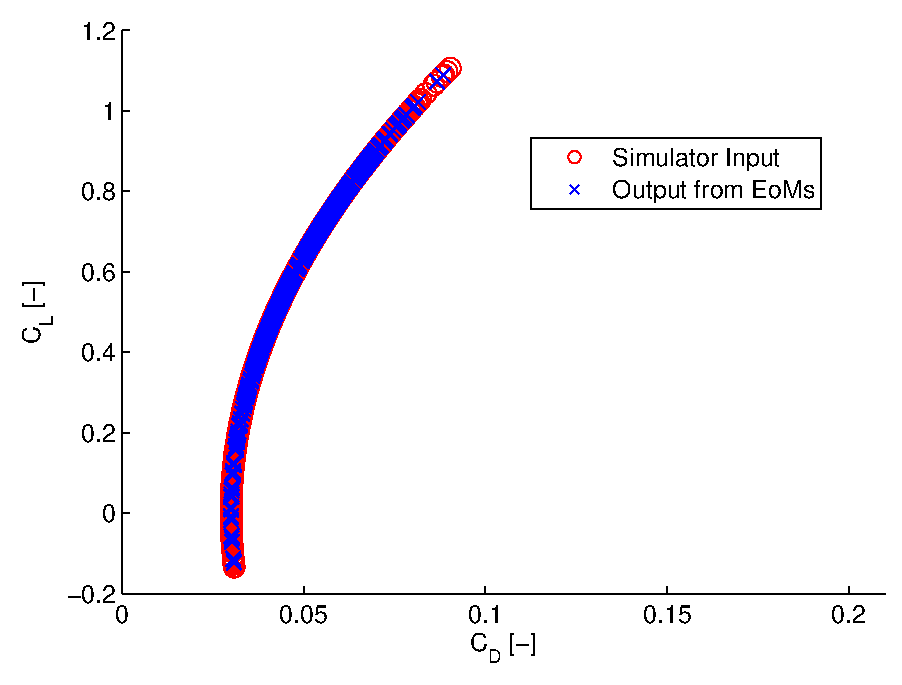
\includegraphics[width=0.5\textwidth]{figures/dragPolarNoNoise.eps}
    \caption{Data Analysis Verification (No Noise)}
        \label{dragPolarNoNoise}
\end{figure}

With this result, noise was added to the system to see how sensitive coefficient estimation was to noise in each sensor. This process was a balancing act between available sensor accuracy and the desired accuracy of the final solution. The final result guided sensor selection to those discussed in Section \ref{hardware}. To check if the final sensors chosen were acceptable, Gaussian noise was added to each state, with a mean of zero and a standard deviation equal to the RMS error listed in the manufacturer's data sheet for each sensor.
\begin{figure}[H]
  \centering
    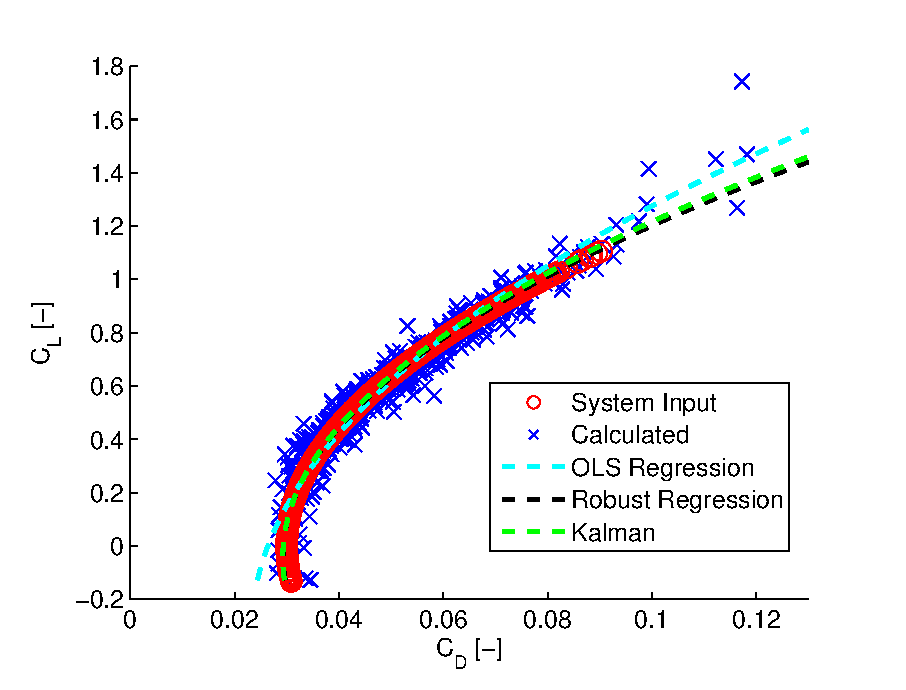
\includegraphics[width=0.5\textwidth]{figures/simDragPolarNoise.eps}
      \caption{Drag Polar Prediction of Simulated Test Flight} \label{dragPolarNoise}
\end{figure}

For the particular simulated test flight shown in Figure \ref{dragPolarNoise}, the estimated drag polar coefficients are shown in Table \ref{simCoeffErrorTable}.

\begin{table}[ht]
\caption{Nonlinear Model Results}
\label{simCoeffErrorTable}
\centering
\begin{tabular}{c c c c}
\hline\hline
 & $C_{D_0}$ & $C_1$ & $C_2$ \\
 \hline
System Inputs & 0.0493 & 0 & 0.03 \\
OLS Estimate & 0.0300 & 0.0196 & 0.0264 \\
Robust LS Estimate & 0.0461 & 0.0034 & 0.0294 \\
Kalman Estimate & 0.0446 & 0.0039 & 0.0293 \\
\hline
\end{tabular}
\end{table}
\nomenclature{OLS}{Ordinary least squares}
\nomenclature{$K_2$}{Drag polar coefficient for $C^2_L$ terms}

The results of this simulated flight test showed that the measurement system outlined in Section \ref{hardware} predicted the simulated drag polar with a reasonable error. It also demonstrates
 the necessity of the heteroskedasticity correction, as the OLS regression has a 65\% error on $K_2$ and a 13\% error on $C_{D_0}$, while the robust regression has a 7\% error on $K_2$ and a 2\% error on $C_{D_0}$.

Since adding random noise results in stochastic error estimates, a Monte Carlo simulation was conducted to quantify expected accuracy values using the sensors selected in Section \ref{hardware}. Error with a standard deviation equal to those reported by the manufacturer was added to clean simulated flight data, and the percent error in each coefficient was saved. This process was repeated 10,000 times, and the results are shown in Figures \ref{fig:cd0monteCarlo}-\ref{fig:c2monteCarlo}.
\begin{figure}[H]
  \centering
    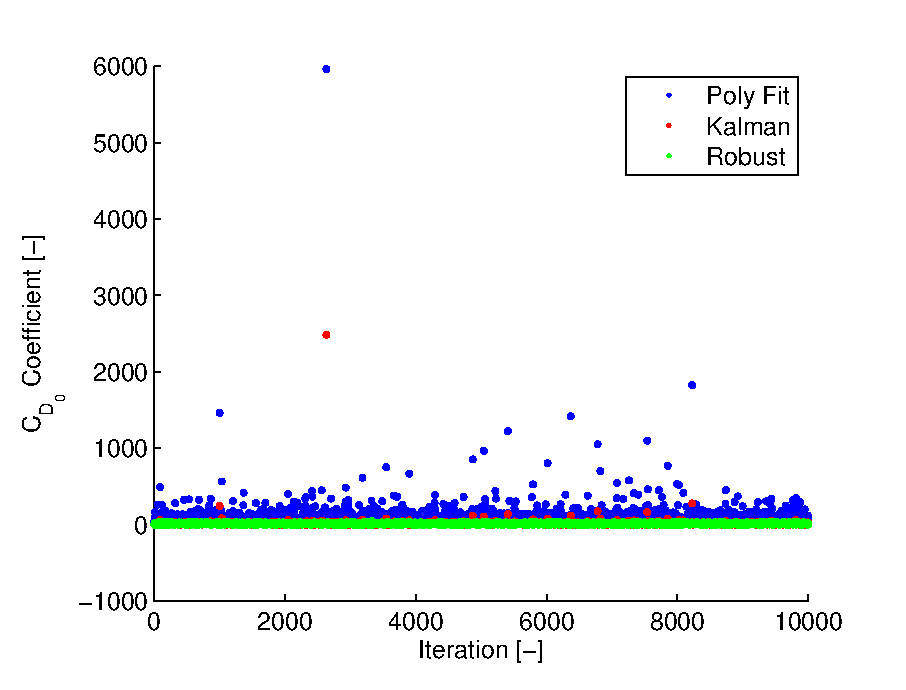
\includegraphics[width=0.5\textwidth]{figures/cd0monteCarlo.eps}
      \caption{$C_{D_0}$ Monte Carlo Simulation}
      \label{fig:cd0monteCarlo}
\end{figure}

\begin{figure}[H]
  \centering
    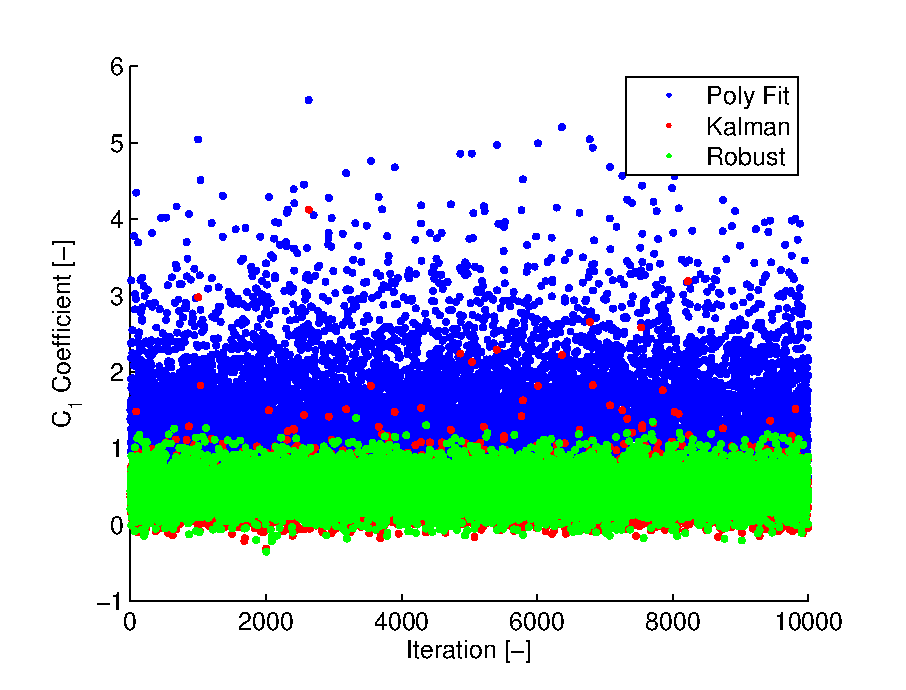
\includegraphics[width=0.5\textwidth]{figures/c1monteCarlo.eps}
      \caption{$C_1$ Monte Carlo Simulation}
      \label{fig:c1monteCarlo}
\end{figure}

\begin{figure}[H]
  \centering
    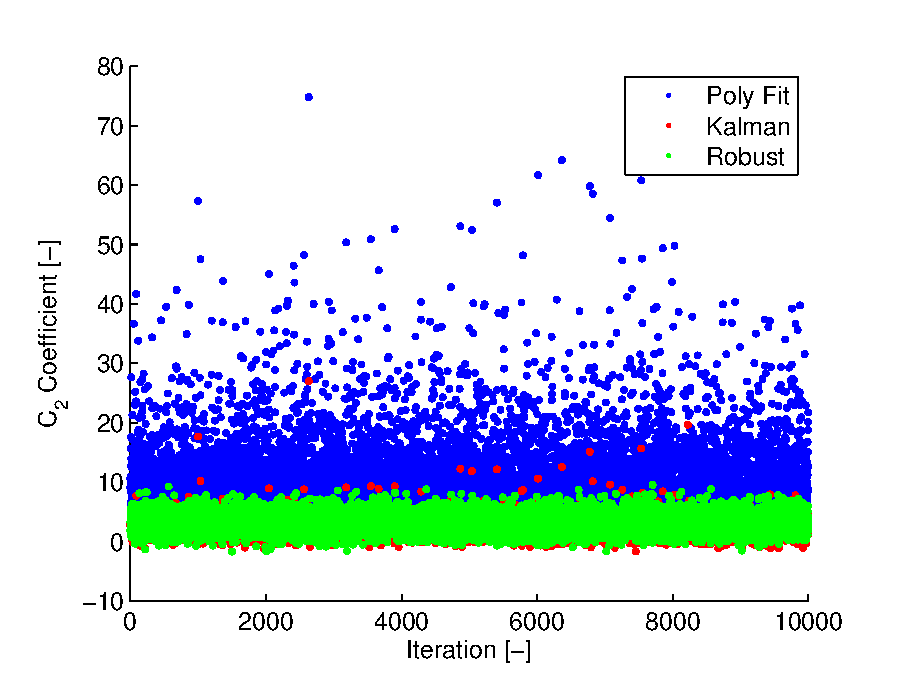
\includegraphics[width=0.5\textwidth]{figures/c2monteCarlo.eps}
      \caption{$C_2$ Monte Carlo Simulation}
      \label{fig:c2monteCarlo}
\end{figure}

The results of the study, summarized in Table \ref{table:monteCarlo}, show that the \texttt{robustfit} regression produced the most accurate and reliable results.

\begin{table}[ht]
\caption{Monte Carlo Results}
\label{table:monteCarlo}
\centering
\begin{tabular}{*7c}
\hline\hline
 &  \multicolumn{3}{c}{Mean Percent Error} & \multicolumn{3}{c}{Percent Standard Error}\\
 & $C_{D_0}$ & $C_1$ & $C_2$ & $C_{D_0}$ & $C_1$ & $C_2$\\
 \hline
OLS & 53.8 & 1.5 & 10.6 & 81.7 & 0.6 & 6.0\\
Robust LS & 12.2 & 0.5 & 3.2 & 6.3 & 0.2 & 1.5\\
Kalman Filter & 12.1 & 0.4 & 2.5 & 26.0 & 0.2 & 1.3\\
\hline
\end{tabular}
\end{table}